%% =============================================================================
%% Executive Summary -- standalone document (separate to the main report).
%% Compile with pdfLaTeX (2 passes for \ref/\cite; no BibTeX needed -- the
%% bibliography is a manual thebibliography). Figures sit next to this file.
%% Target: <= 1000 words (body). Audience: numerate non-specialist.
%% =============================================================================
\documentclass[10pt,a4paper,twocolumn]{article}

\usepackage[utf8]{inputenc}
\usepackage[T1]{fontenc}
\usepackage[margin=1.9cm]{geometry}
\usepackage{microtype}
\usepackage{graphicx}
\graphicspath{{./}}
\usepackage{float}
\usepackage{booktabs}
\usepackage{caption}
\usepackage{titlesec}
\usepackage{enumitem}
\usepackage[most]{tcolorbox}

% slightly heavier text: render the default (medium) series in the bold weight
\renewcommand{\mddefault}{b}
\captionsetup{font=footnotesize,labelfont=bf}
\titleformat{\section}{\normalfont\large\bfseries}{}{0pt}{}
\titlespacing*{\section}{0pt}{1.0ex}{0.4ex}
\setlength{\parskip}{0.35ex}
\pagestyle{empty}

\begin{document}

\twocolumn[{%
  \centering
  {\large\bfseries PRESERVING RARE-CLASS SIGNAL IN FEDERATED LEARNING\par}
  \vspace{0.3em}
  {\normalsize\bfseries\scshape Under Statistical and System Heterogeneity\par}
  \vspace{0.55em}
  {\small\scshape Barbara Koch \quad$\vert$\quad MPhil Data Intensive Science \quad$\vert$\quad University of Cambridge\par}
  \vspace{1.4em}
}]

\section*{Why This Project Matters}
Accurate diagnostic models need large, diverse image collections, but in medicine
those images are scattered across hospitals and usually cannot be pooled because of
privacy law. \emph{Federated learning} (FL) offers a way out~\cite{rieke2020future}:
each site keeps its data and shares only model updates, which a central server merges
into one global model. Two practical problems make this hard in medicine. Sites see
different case mixes (\emph{statistical heterogeneity}), and they differ in compute
and availability (\emph{system heterogeneity}), so some sites return only partial work
in a given round. Medical image data is also severely class-imbalanced: a few benign
conditions dominate, while the urgent diagnoses are rare. The worst case is when the
slow or under-resourced site is the one holding the rare disease. A model can then
report high overall accuracy while quietly failing on exactly the lesions that matter
clinically. Crucially, the information needed to recognise a rare disease reaches the
shared model only through the updates of the site that holds it --- so the algorithm
that \emph{merges} those updates, not the network architecture, decides whether that
rare-disease signal survives (Figure~\ref{fig:flow}).

\begin{figure}[H]
\centering
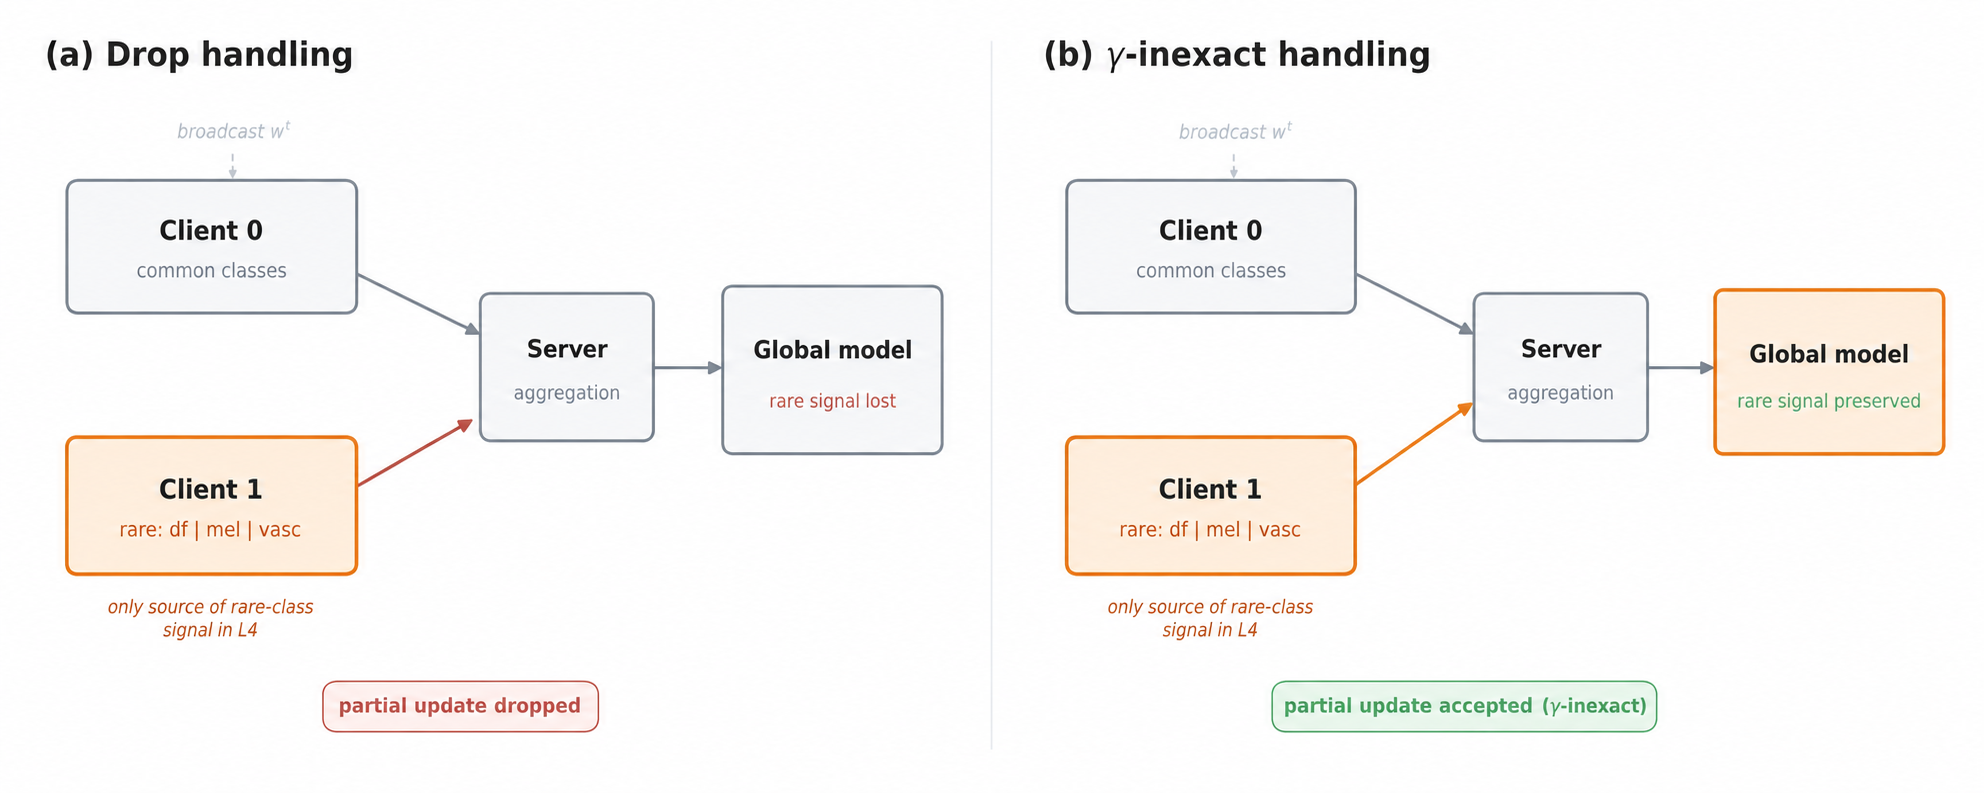
\includegraphics[width=\linewidth]{F_signal_flow_gamma_inexact_improved.png}
\caption{How a slow rare-class site's update is handled. Discarding the partial
update (a) loses the rare-disease signal; accepting it (b) lets that signal reach the
global model --- the mechanism behind the headline result.}
\label{fig:flow}
\end{figure}

\section*{Approach}
We studied this on DermaMNIST~\cite{yang2023medmnistv2}, a seven-class dermatology
benchmark of small ($28\times28$) skin-lesion images~\cite{tschandl2018ham10000} in
which benign moles make up two-thirds of the data and the urgent classes, including
melanoma, are rare. Using controlled, simulated federations, we compared the three
most widely used FL merging algorithms --- FedAvg~\cite{mcmahan2017fedavg},
FedProx~\cite{li2020fedprox} and FedNova~\cite{wang2020fednova} --- and asked not
``which is best?'' but ``in which conditions does each preserve or lose rare-disease
performance?'' We scored models by \emph{macro-F1}, which weights all seven classes
equally and therefore exposes the rare-class failure that raw accuracy hides. We then
varied one factor at a time: how data is split across sites, whether a slow site's
partial update is discarded or accepted, how strongly a site's learning is weakened,
and whether the training loss is rebalanced. The sharpest test used two matched
two-client federations differing in only one respect --- whether the slow site
uniquely holds the rare diseases --- so any performance gap cleanly isolates the value
of admitting that unique signal. A single idea organises the work ---
\emph{rare-client signal flow}: a rare disease is learned only to the extent that the
holding site's contribution reaches and persists in the global model.

\section*{Key Findings}
Differences between the algorithms are small until the right stress is applied
(Table~\ref{tab:regime}). With balanced participation, FedProx and FedAvg differ by
under $0.01$ macro-F1, and FedProx's one tuning knob helps only in a narrow range ---
pushed an order of magnitude too high it costs $0.074$ macro-F1 and damages precisely
the rare classes. The central result concerns slow
sites (``stragglers''). When the rare-disease site is the straggler, the
FedProx~$+$~$\gamma$-inexact protocol beats FedAvg~$+$~drop by a large $+0.115$
macro-F1; but a controlled decomposition shows that about $96\%$ of that gain
($+0.111$) traces to the $\gamma$-inexact handling that \emph{accepts} the slow site's
partial update --- the protocol conventionally paired with FedProx here --- and almost
none ($+0.004$) to the proximal regularisation term itself. A matched control in which
the slow site holds nothing unique erases the effect, confirming the mechanism is the
admission of rare-disease signal, not the algorithm's branding. Under an extreme
``perfect storm,'' the FedProx~$+$~$\gamma$-inexact protocol reaches $0.49$ macro-F1
where FedAvg~$+$~drop collapses to $0.09$ (Figure~\ref{fig:gaps}). FedNova proved regime-dependent: robust when a site is
steadily weakened (leading by $+0.131$ in the most extreme case) but collapsing to
$0.24$ under random, round-to-round slowness. Every failure shared one signature ---
rare lesions misrouted into the benign majority class (in one cell, melanoma was
recovered $1\%$ of the time by FedAvg versus $46\%$ by FedNova). Finally, simply
reweighting the training loss matched FedProx, showing that imbalance correction is a
separate lever from update merging.

\begin{figure}[H]
\centering
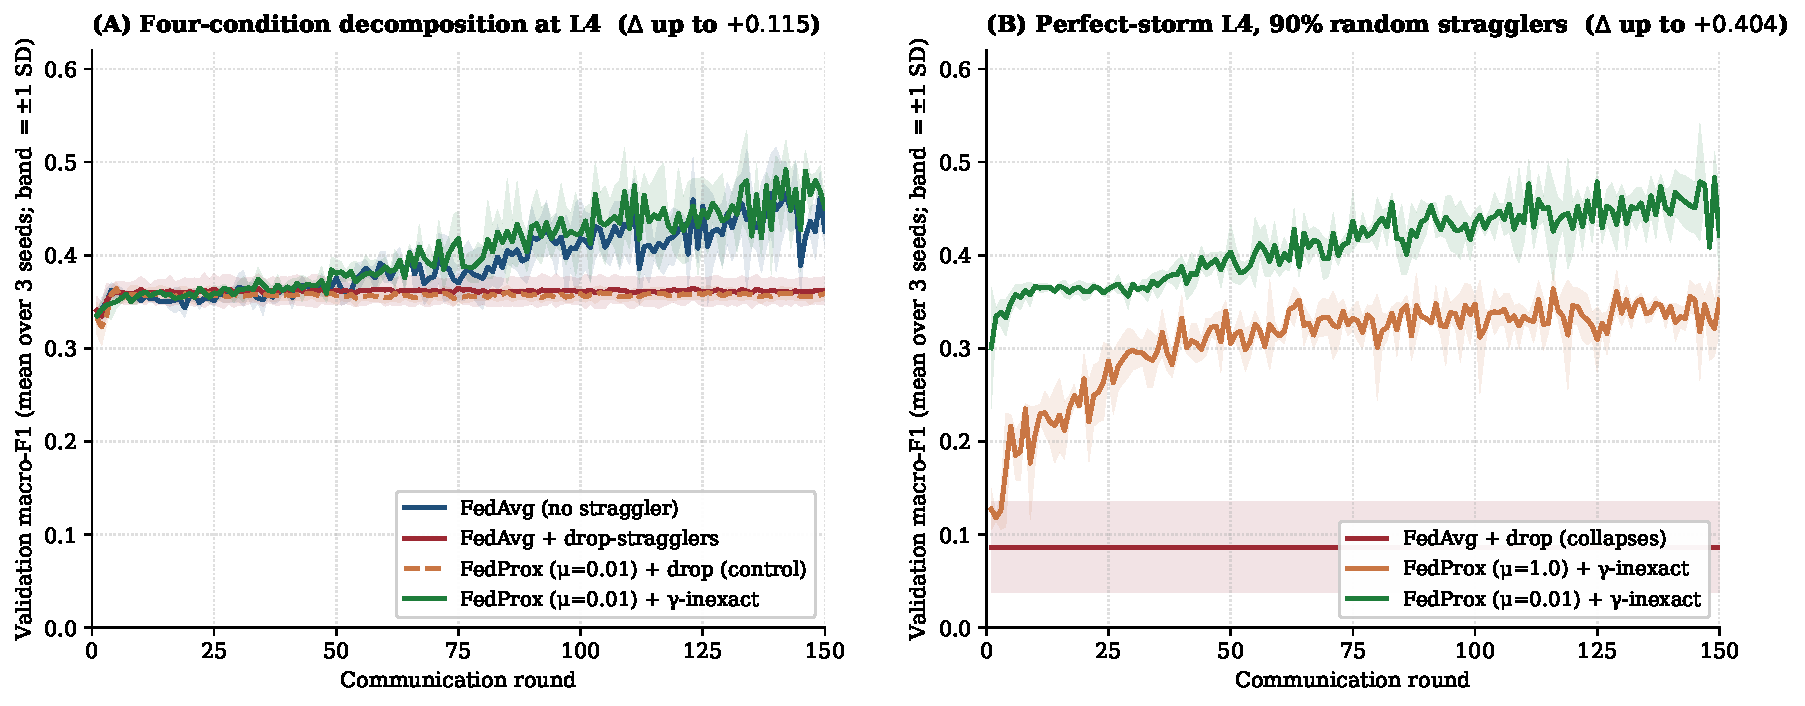
\includegraphics[width=\linewidth]{F_val_curves_extreme_gaps.pdf}
\caption{Validation macro-F1 over training at the two largest gaps. Under the
FedProx~$+$~$\gamma$-inexact protocol the slow site's partial update is accepted and
rare-class performance recovers; the FedAvg~$+$~drop protocol discards it and
flatlines.}
\label{fig:gaps}
\end{figure}

\begin{table*}[t]
\centering
\caption{Regime map: which mechanism preserves rare-class signal, and the supporting
macro-F1 evidence. There is no universal winner --- the protective mechanism changes
with the heterogeneity regime.}
\label{tab:regime}
\small
\begin{tabular}{p{0.30\textwidth} p{0.34\textwidth} p{0.28\textwidth}}
\toprule
Heterogeneity regime & What preserves rare-class signal & Macro-F1 evidence \\
\midrule
Balanced / IID participation        & No method needed (all comparable)                 & $\Delta \approx 0$ (IID $-0.007$) \\
Statistical heterogeneity only       & Weak FedProx edge                                 & $\Delta \approx +0.007$ \\
Straggler drops the rare-class site  & \textbf{Accepting} the partial update (FedProx~$+$~$\gamma$-inexact) & $+0.115$ total; $96\%$ from acceptance, $4\%$ from the proximal term \\
``Perfect storm'' (90\% random stragglers) & Accepting partial updates                   & $0.49$ vs $0.09$ when dropped \\
Steady learning-rate weakening       & FedNova (work-normalised merging)                 & leads by $+0.131$ at $50{:}1$ \\
Random, round-to-round slowness      & None robust; FedNova collapses                    & $0.24$ (majority-only) \\
\bottomrule
\end{tabular}
\end{table*}

\begin{figure*}[t]
\centering
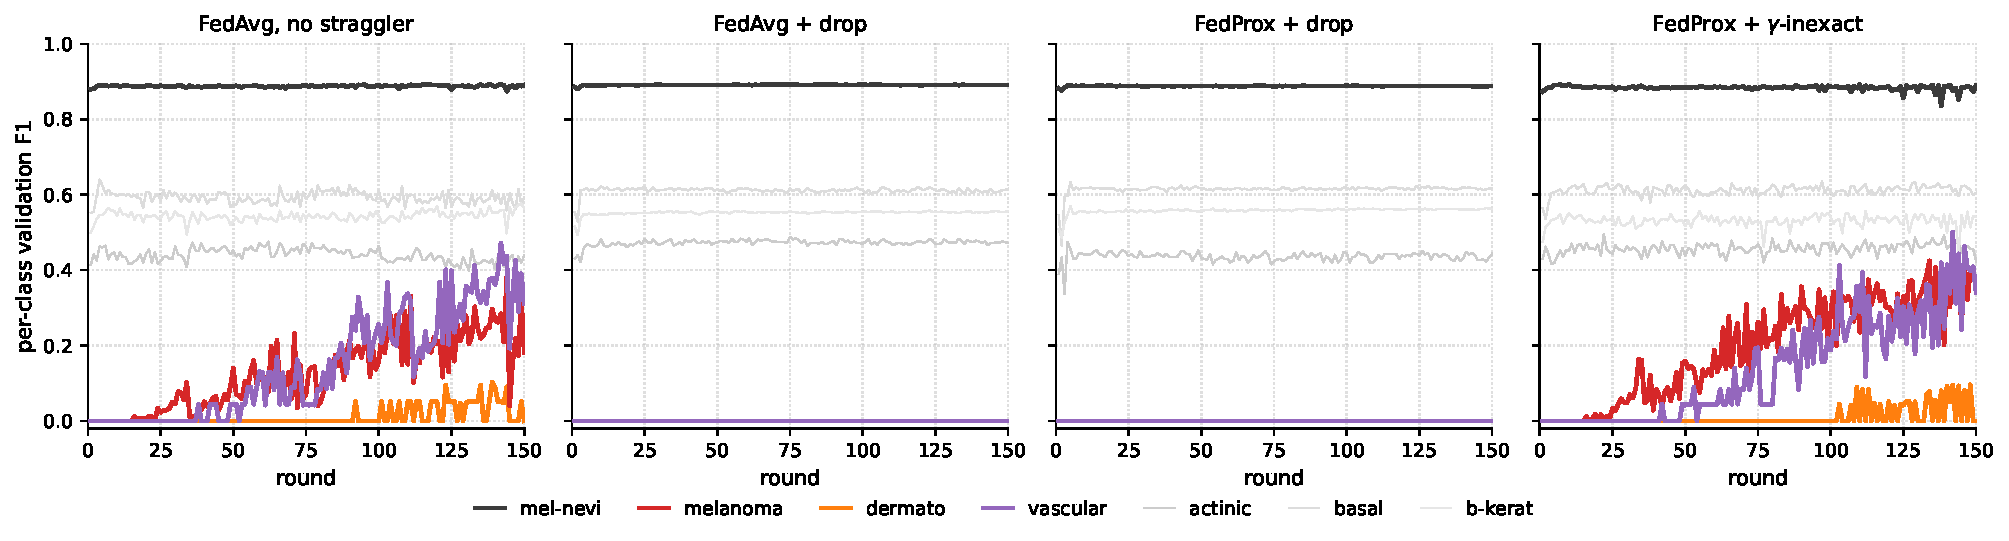
\includegraphics[width=\textwidth]{F_l4_four_condition_per_class_grid.pdf}
\caption{Per-class validation F1 under the four-condition decomposition. The majority
class is unaffected, but the three rare classes flatline under \emph{both} drop
conditions and recover \emph{only} when the partial update is accepted
(FedProx~$+$~$\gamma$-inexact) --- pinpointing rare-class learning as the locus of the
effect.}
\label{fig:grid}
\end{figure*}

\section*{Interpretation \& Impact}
All of these results reduce to one rule: rare-class performance is preserved
precisely when rare-site signal reaches the global model with usable weight. This
reframes a crowded methods debate. There is no universal best FL optimiser; the right
choice is dictated by the heterogeneity regime, and the decisive factor is often a
protocol detail --- whether partial updates are admitted --- rather than the headline
algorithm. For anyone building imbalanced medical FL systems the practical guidance
follows directly from the regime, summarised in the box below. The contribution is a
regime map and a mechanism --- conceptually relevant beyond dermatology, and worth
testing in other rare-class federated settings.

\section*{Next Steps}
The most promising extension is to combine partial-update acceptance with loss
rebalancing, which were effective separately here. Beyond that: validate the map on
higher-resolution, genuinely multi-site data with real wall-clock deadlines; broaden
the comparison to variance-reduced and adaptive optimisers; and log per-site
performance to quantify fairness across hospitals --- but the mechanism isolated here
is exactly the one a real deployment must protect.

\begin{figure}[H]
\centering

\includegraphics[width=0.78\linewidth]{F_asymmetric_lr_L4.pdf}
\caption{FedNova: robust to steady weakening, brittle under random stragglers.}
\label{fig:lr}
\end{figure}

\begin{tcolorbox}[enhanced, sharp corners, boxrule=0.5pt, colframe=black!80,
  colback=white, coltitle=black, colbacktitle=black!10,
  fonttitle=\bfseries\footnotesize, title=What This Means in Practice,
  toptitle=2.5pt, bottomtitle=2.5pt, left=6pt, right=6pt, top=4pt, bottom=4pt,
  boxsep=1pt]
{\footnotesize
\begin{itemize}[leftmargin=1.2em,itemsep=3pt,topsep=2pt,parsep=0pt,label=\textbullet]
\item \textit{Near-IID clients} --- FedAvg is enough.
\item \textit{Statistical heterogeneity alone} --- the FedProx edge is small and fragile.
\item \textit{Rare-class site straggling} --- accepting its partial update
  (FedProx~$+$~$\gamma$-inexact) is the key protection.
\item \textit{Rare site steadily weakened} --- FedNova's work-normalised merging can help.
\item \textit{Random round-to-round straggling} --- do not assume FedNova is safe.
\item \textit{Reporting} --- use macro-F1 and per-class/rare-class metrics, never accuracy
  alone.
\end{itemize}}
\end{tcolorbox}

\smallskip
\noindent{\footnotesize\emph{Scope and caveats.} A single $28\times28$ DermaMNIST
benchmark; simulated heterogeneity; mechanism probes at $n=3$ seeds; clinically
motivated, not validated. The straggler gain is attributed to the
FedProx~$+$~$\gamma$-inexact \emph{protocol}, not to partial-update acceptance as a
proven standalone mechanism.}

{\footnotesize
\begin{thebibliography}{9}
\setlength{\itemsep}{0pt}
\bibitem{rieke2020future} N.~Rieke et al. The future of digital health with federated learning. \emph{npj Digital Medicine}, 3:119, 2020.
\bibitem{yang2023medmnistv2} J.~Yang et al. MedMNIST v2 --- A large-scale lightweight benchmark for 2D and 3D biomedical image classification. \emph{Scientific Data}, 10:41, 2023.
\bibitem{tschandl2018ham10000} P.~Tschandl, C.~Rosendahl, H.~Kittler. The HAM10000 dataset of dermatoscopic images of pigmented skin lesions. \emph{Scientific Data}, 5:180161, 2018.
\bibitem{mcmahan2017fedavg} B.~McMahan et al. Communication-efficient learning of deep networks from decentralized data. \emph{AISTATS}, 2017.
\bibitem{li2020fedprox} T.~Li et al. Federated optimization in heterogeneous networks (FedProx). \emph{MLSys}, 2020.
\bibitem{wang2020fednova} J.~Wang et al. Tackling the objective inconsistency problem in heterogeneous federated optimization (FedNova). \emph{NeurIPS}, 2020.
\end{thebibliography}
}

\end{document}
